\chapter{\uppercase {\crossflowcap Implementation}}
\label{sec:evaluation}

\section{Illustrative \crossflow Implementation}

In this section, we describe our implementation of \emph{adaptive modulation}, \emph{frequency hopping} and \emph{cognitive radio} applications using the \crossflow framework. For illustration, we implement our model on a USRP N210 embedded SDR from Ettus Research. The N210 provides a Zynq 7020 All Programmable SoC, which combines a dual ARM Cortex-A9 processor and FPGA on the same device. We use the CPqD Softswitch~\cite{ofsoftswitch13} (\texttt{ofsoftswitch}) software as the switch agent in the SDN model. Its main functionality is to enable communication between GNU Radio and the python based Ryu SDN controller. As described in previous sections, the applications will send messages to the processing blocks, e.g., to configure them. The \texttt{ofsoftswitch} then forwards this request to a centralized \texttt{\crossflow Hub} inside the GNU Radio domain. 

%The responsibility of this block is to switch the request according to the specified processing block. In our current model shown in Figure~\ref{fig:message_block}, we implement the interface requirements for two blocks: Modulators and Sink. The \texttt{Mod Controller} and \texttt{USRP Controller} blocks are responsible for translating the request messages into implementable actions for the processing blocks and also reporting the responses from the blocks to \texttt{CrossFlow Hub} for certain events supported by the blocks. In the current version, we are capable of providing configuration capability to the applications and we will soon incorporate event reporting and sensing capability into the implementation.
\begin{figure}[t]
  \centering
  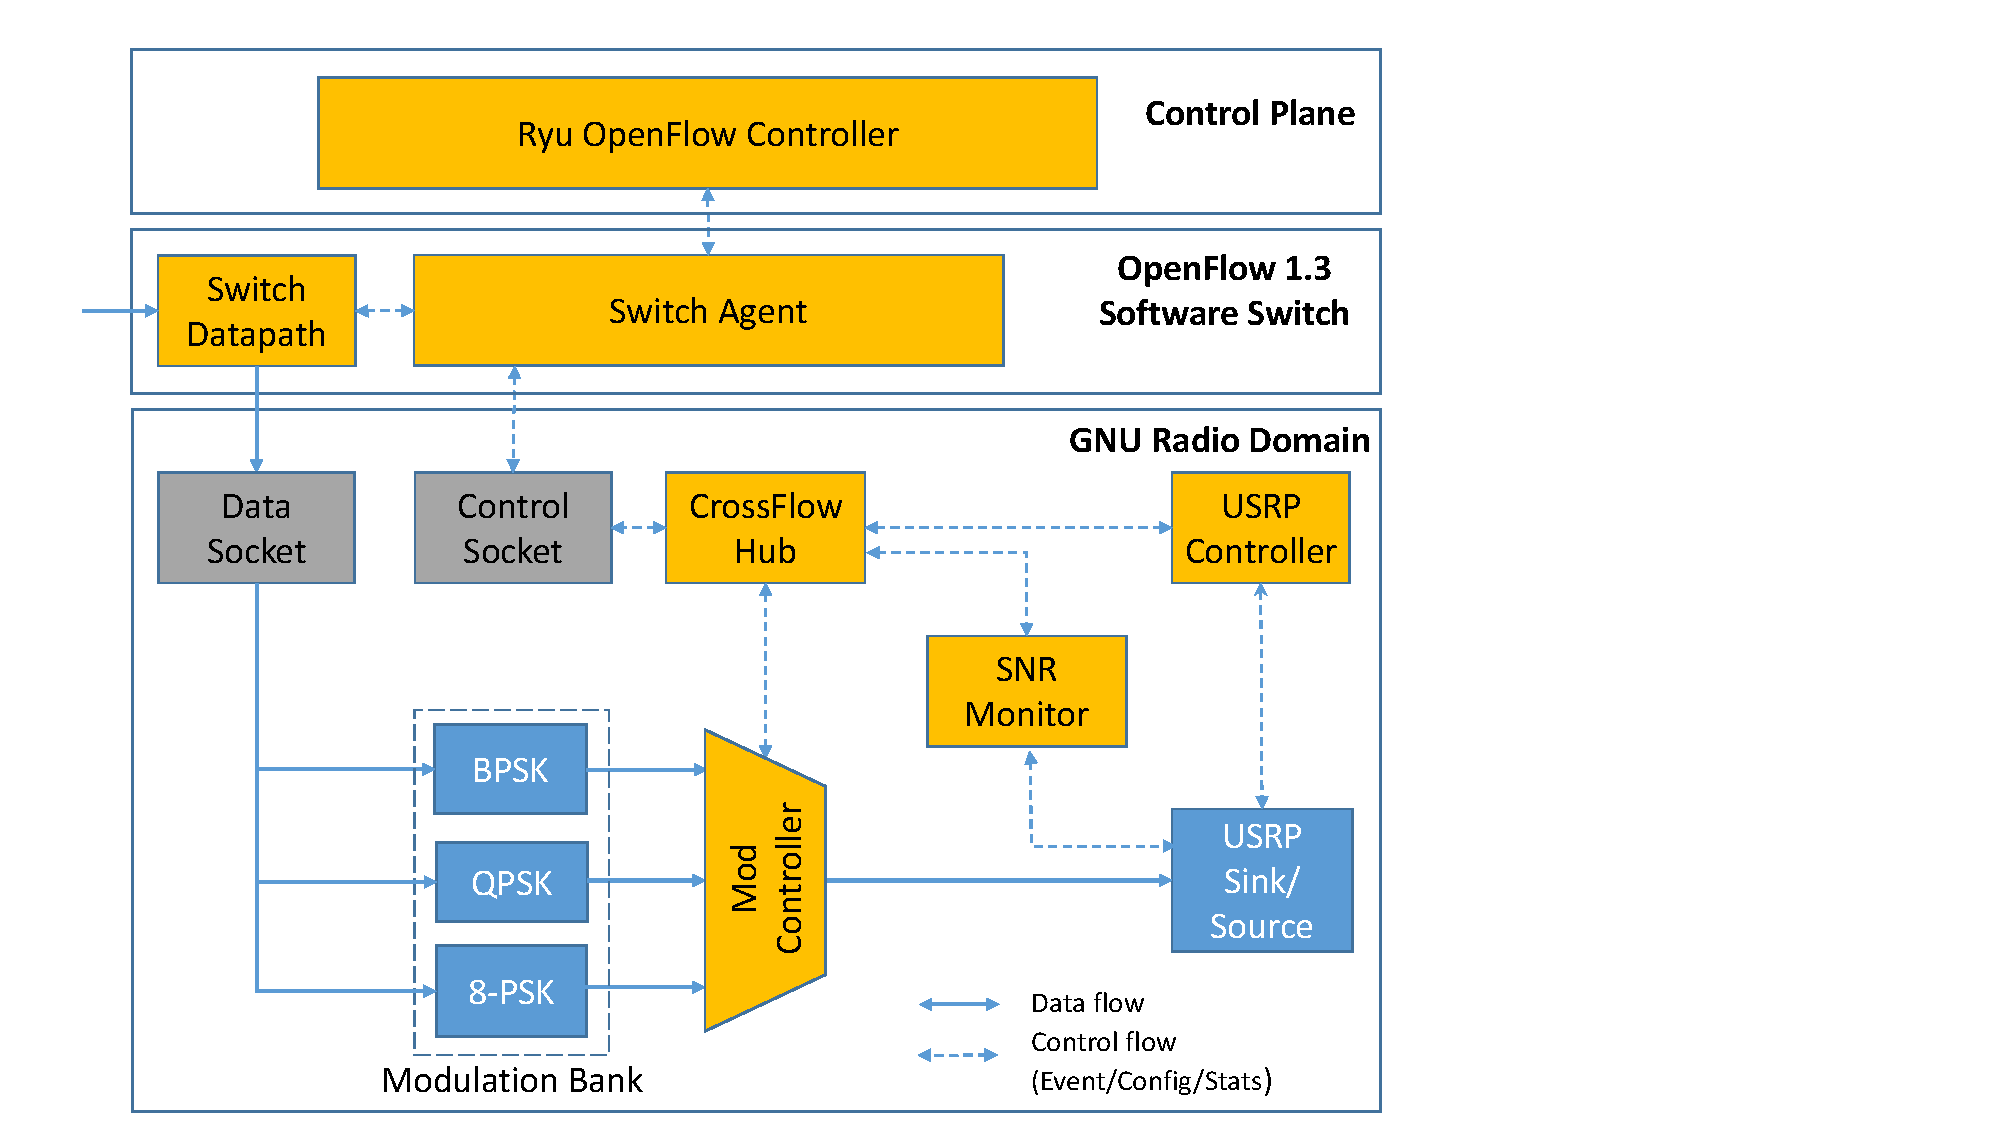
\includegraphics[width=0.8\textwidth]{figures/Flowgraph.pdf}
  \caption{Transmitter implementation diagram of \crossflow with two processing blocks: Sink and Modulators.}
  \label{fig:flowgraph}
\end{figure}

There are four main components (blocks) in the illustrative \crossflow module, as given in Figure~\ref{fig:flowgraph}, that we implement in GNU Radio, namely, the \texttt{\crossflow Hub}, the Modulation Controller (Mod Controller for brevity), and the USRP Controller.
\begin{itemize}
\item The \texttt{\crossflow Hub} is the interface between the Mod and USRP controllers in GNU Radio and the Ryu SDN controller. The \texttt{\crossflow Hub} and the Ryu SDN controller communicate via Socket PDU. The \texttt{\crossflow Hub} is responsible for receiving commands from \texttt{ofsoftswitch} (or any other compliant interface), interpreting the commands, and forwarding the commands to the appropriate controller block (i.e., either the USRP controller or Mod controller in our implementation). It is also responsible for receiving information from different controller blocks and sending information to the Ryu SDN controller. The \texttt{\crossflow Hub} has in/out ports to send commands and receive information to/from the GNU radio controller blocks. It also has in/out PDU ports for interfacing with Socket PDU.
\item The Mod Controller is one of the main controllers in the design. It is responsible for receiving commands from the \texttt{\crossflow Hub}, and selecting the appropriate modulation scheme from the modulation bank. For illustration, we include three modulation schemes in our modulation bank (BPSK, QPSK, and 8PSK); however, thanks to the modular design, we can easily add more schemes. The Mod Controller can also feedback information to the Ryu SDN controller about the modulation scheme that is currently in use and the number of modulation schemes available in the modulation bank.
\item The \texttt{SNR Monitor} is responsible for monitoring the SNR level and generating an event in case the SNR level falls below a certain threshold, which can be configured by the application. Currently the framework uses the existing SNR probe of GNU Radio, which supports four $M$-PSK SNR estimators. This monitoring block is also responsible for relaying the SNR statistics back to \texttt{\crossflow Hub} in response to a SNR statistics query generated by the application.
\item The USRP Controller is another controller block in the \crossflow module. It is responsible for controlling different RF parameters of the USRP Transmitter/Receiver based on commands from the \texttt{\crossflow Hub}. In our proof-of-concept implementation, we control the carrier frequency and the power of the signal. It can also feedback information to the \texttt{\crossflow Hub} about the current RSSI, temperature, SNR, carrier frequency, power, etc.
\end{itemize}
Although our illustrative implementation only has two controllers (one facilitating abstraction of the USRP Sink/RF implementation and the other facilitating abstraction of the adaptive modulation implementation), additional controllers can be easily added to support new applications, functionalities, and abstractions.
%As we mentioned before, for this implementation, we have two controllers, but its design is modular, and more controllers can be added easily to support new applications/functionality.

\section{Example Applications}


\subsection{Frequency Hopping Application}
Frequency hopping is a technique of transmitting radio signals by spreading the signal over a sequence of changing frequencies. It has tremendous application in military as it is used against jamming and for protecting against unauthorized eavesdropping. For implementation, the receiver of the signal must be aware of the sequence of frequencies so that it can tune into the appropriate channel. This requires synchronization between the transmitter and the receiver. In \crossflow, we implement this application easily as only the controller needs to be aware about the predetermined sequence. This sequence can even be dynamic according to the channel conditions and policies.   

\subsection{Adaptive Modulation Application}
Adpative Modulation is a technique where the modulation is changed according to the conditions of the channel. There are various estimators which are used for obtaining channel quality. These can be Signal-to-noise ratio (SNR), Bit error rate (BER) and other environment specific estimators. For illustration, we assume a fixed sequence for changing the modulation schemes every 5 seconds. 

\subsection{Cognitive Radio Application}
We build upon the frequency hopping application mentioned above to construct a cognitive radio application. Cognitive radio is a type of radio in which the device is aware of its environment and can dynamically change its operating parameters like transmission power, frequency, gain etc in response to changing environmental conditions. In \crossflow, we implement an application that can configure a radio device to switch channels based upon a low SNR event measured by the device.
